% ----------
% A LaTeX template for course project reports
% 
% This template is modified from "Tech Report ala MIT AI Lab (1981)"
% 
% ----------
\documentclass[12pt, letterpaper, twoside]{article}
\usepackage{geometry}
\usepackage[utf8]{inputenc}
\usepackage[english]{babel}
\usepackage[runin]{abstract}
\usepackage{titling}
\usepackage{booktabs}
\usepackage{fancyhdr}
\usepackage{helvet}
\usepackage{csquotes}
\usepackage{graphicx}
\usepackage{blindtext}
\usepackage{parskip}
\usepackage{etoolbox}
\usepackage{hyperref}

\graphicspath{ {./resources/report_pics/} }


% preamble.tex

\geometry{letterpaper, top=2.2in, headheight=1.7in}
\date{}

\makeatletter

\def\fulltitle#1{\def\@fulltitle{#1}}
\def\runningtitle#1{\def\@runningtitle{#1}}
\def\runningauthor#1{\def\@runningauthor{#1}}
\def\affiliation#1{\def\@affiliation{#1}}
\def\department#1{\def\@department{#1}}
\def\memoid#1{\def\@memoid{#1}}
\def\theyear#1{\def\@theyear{#1}}
\def\mydate#1{\def\@mydate{#1}}

\runningtitle{How to write an effective report} % Short title
\author{Your name \and John Doe \and Jane Doe} % Full list of authors
\runningauthor{Your name et al.} % Short list of authors
\affiliation{Your University} % Affiliation e.g. University or Company
\department{Your Department} % Department or Office
\memoid{AI Memo 777} % ID of the tech report
\theyear{2018} % year of the tech report
\mydate{August 08, 2018} %the date

\def\displaymydate{\@mydate}
\def\displaytheyear{\@theyear}
\def\displaymemoid{\@memoid}
\def\displaydepartment{\@department}
\def\displayaffiliation{\@affiliation}
\def\displayrunningauthor{\@runningauthor}
\def\displayrunningtitle{\@runningtitle}

\makeatother

\makeatletter
\patchcmd{\@zfancyhead}{\fancy@reset}{\f@nch@reset}{}{}
\patchcmd{\@set@em@up}{\f@ncyolh}{\f@nch@olh}{}{}
\patchcmd{\@set@em@up}{\f@ncyolh}{\f@nch@olh}{}{}
\patchcmd{\@set@em@up}{\f@ncyorh}{\f@nch@orh}{}{}
\makeatother

% ----------
% fancyhdr setup
% ----------

\pagestyle{fancy}
\renewcommand{\headrulewidth}{0pt}

\fancypagestyle{firstpage}
{
    \fancyhf{}
    \fancyhead{%
        \begin{center}
            \textsc{\displayaffiliation}\\
            \textsc{\displaydepartment}
        \end{center}
        \vspace*{0.5in}
        \displaymemoid
        \hfill
        \displaymydate
    }
    \fancyfoot[L]{\footnotesize \textbf{\textsc{\displayaffiliation} -- \displaytheyear}}
}
\fancyhead[EL]{\small \displayrunningauthor}
\fancyhead[ER]{\small Page \thepage}
\fancyhead[OL]{\small Page \thepage}
\fancyhead[OR]{\small \displayrunningtitle}

\chead{}
\lfoot{}
\cfoot{}
\rfoot{}

% ----------

\providecommand{\keywords}[1]{\noindent \textbf{Keywords:} #1} % keywords definition

\renewcommand{\familydefault}{\sfdefault} % sans-serif font
\setlength{\parskip}{1em} % 1em skip between paragraphs
\abslabeldelim{:} % use colon after the run-in 'Abstract' word
\setlength{\parindent}{0pt} % no indentantion for first page 
\setlength{\abstitleskip}{-\absparindent} % this is because the abstract package sets \absparindent to \parindent

\pretitle{\Large \begin{center}}
\posttitle{\\[2ex] \Large \textbf{by}\end{center}}

% ----------
% Variables
% ----------

\title{\textbf{Helping Municipalities Maintain Roads by Locating Defects Using Computer Vision}} % Full title of your tech report
\runningtitle{Detecting Road Defects Using Computer Vision} % Short title
\author{Samuel Bazinet} % Full list of authors
\runningauthor{Samuel Bazinet} % Short list of authors
\affiliation{Ontario Tech University} % Affiliation e.g. University or Company
\department{Faculty of Science, Computer Science} % Department or Office
\memoid{Project} % Project group ID that were shared with the class earlier.
\theyear{2024} % year of the tech report
\mydate{April 5, 2024} %the date


% ----------
% actual document
% ----------
\begin{document}
\maketitle

\begin{abstract}
    \noindent
    
    In a world where efficiency is more important than ever and with roads being built all the time,
    finding road defects needs to be as automated as possible to maintain a good driving experience for all citizens. 
    With computers getting faster by the year, 
    we can use this newfound ability to use them to help us automatically find defects such as potholes and cracks without human intervention.
    This paper looks over how we can setup such a system, 
    including finding an algorithm to find potential defects, 
    as well as training a machine learning model to differentiate between the types of defects.

    % Uncomment the following to add keywords as needed
    \keywords{Computer Vision, Infrastructure}
\end{abstract}

\vspace{2.5cm}

% Uncomment the following to add thanks.
% {\footnotesize
%     \noindent
%     Special thanks to \textbf{Person 1} and \textbf{Affiliation A} for financial support for this project.
% }

\thispagestyle{firstpage}

\pagebreak

% ----------
% End of first page
% ----------

\newgeometry{} % Redefine geometries (normal margins)

\section{Introduction}
\label{sec:intro}

This course on computer vision started with a lab where stop signs had to be identified on an image. 
This was relatively simple as stop signs are standardized so they can be easily identified. 
Unfortunately, the same cannot be said for road defects. 
We cannot simply use a single default template and expect to get a substantial true match rate. 
This means that a substantial amount of work needs to take place in order to be able to outline the potential defects on the road.
This paper will go over the efforts required to get a relatively competent model to detect defects on an image of a road. 

\section{Methodology}
\label{sec:meth}

Detecting defects on a road is a somewhat complex procedure involving many steps to get the model going. 
As we are trying to find cracks and potholes, we cannot use simple pattern matching as they very a lot in size, color, and pattern.
We need a machine learning model for this.
To achieve the model, a dataset will need to be created, then the model will be trained, before being used to highlight the defects on images.

\subsection{Finding Potential Defects}
\label{sec:meth:1}

The first part of finding defects on road is to scan the image for potential defects. 
Cracks and potholes tend to be very well defined on roads, meaning that Canny edge detection is great way to find them.
But since roads can contain many edges, a blurring filter is ran beforehands to reduce the noise in the resulting edges.
Then, the program scans the image and groups the edges into their own objects so that we can extract the potential defects as their own images for later usage.
To make this easier, a dataclass called `Defect' was created.
This dataclass contains the coordinates of the corners of the area containing all the edges, as well as a list of pixels of where the edges were detected.
This class has a few helepr methods to merge potential defects contained within each other as the assumption was made that they would be part of the same defect.
It also has a method to ``recenter'' itself around the densest collection of edges for the purpose of training the model with evenly sized images.
50 images of damaged roads were ran through this ``potential defect extractor'' to collect hundreds of potential defects that will be used for training the model that will be used to detect the real defects.
\hyperref[app:train_data]{A subset of those pictures.}

\subsection{Training a Model to Classify the Defects}

There are 3 classes that will be used by the model: crack, pothole, and non-defect. 
To train the model, the images of the potential defects generated by the last step have been manually classified into 3 folders, one for each class.
Keras and TensorFlow were used to train the model as they were easy to use and have plenty of online resources for extra help.
The model consists of 7 layers consisting of rescaling, 2D convolutions, pooling, flattening, and dense.
The data was augmenting using the Keras sequential augmenter, where the data set had images copied with different rotation and zoom levels.
This is quite useful as generating more images for training is very time consuming.
The model was trained over 100 epochs, where the training accuracy went from low 30\% to around 80\%,
and the validation accuracy reached 70\% \hyperref[app:model_plot]{(see plot)}.
The model was saved for access by the actual defect identifier.

\subsection{Applying the model to potential defects and highlighting them on an image}

Using the same method as defined in \hyperref[sec:meth:1]{Section 2.1}, potential defects are found on the target images.
The model is then loaded into the Jupyter notebook and the potential defects are passed through it, where the predictions are obtained.
Using the prediction from the model, we draw a red line around predicted potholes, and a green line around predicted cracks.
Non defects are not highlighted.
This results into an image where the defects are highlighted so that municipalities and whoever need the data will get to use it.

\section{Results}
\label{sec:resu}

The model was tested on \hyperref[app:result_image]{a few pictures} with mixed results. 
The model is somewhat competent at identifying potholes and cracks, but it often mislabels them and misses quite a few defects as well.
It is quite sensitive to the resolution of the images and the low validation accuracy is made quite apparent.

\section{Discussion and Conclusions}
\label{sec:conc}

So is it all the model's fault? 
Quite frankly, the method used to extract potential defaults is not too good as it is sensitive the resolution of the image.
This sensitivity is mostly due to the fact that every potential defect needs to be the same size to work on with the model.
This causes images of higher resolution to have the defect being cropped, thus making it harder for the model to both train and recognize it.
The method also works under the assumption that defects are often near edges detectable by canny edge detection, 
but that method has its limits and affects the potential defect extracted from an image.
The dataset used to train the model only contained a bit over 400 images, 
which is small enough to lead to potential overfitting, despite the currently low accuracy.
This is somewhat mitigated by data augmentation, but that method only goes so far.

Would this model be useful for the target audience?
In this state, not really.
But it is a good fondation that can be built upon by giving it more data and making it less sensitive to the original image resolution.
There were not obvious signs of overfitting in the model, 
so it is possible that more epochs will give a better accuracy,
at the cost of longer training.

\appendix

\section{Sample images used in training the model}
\label{app:train_data}

\subsection{Non defects}
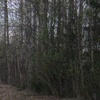
\includegraphics{rd1_0.jpg}
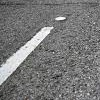
\includegraphics{rd2_9.jpg}

\subsection{Cracks}
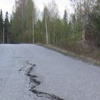
\includegraphics{rd1_3.jpg}

\includegraphics{rd2_2.jpg}

\subsection{Potholes}
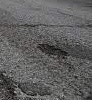
\includegraphics{rd2_5.jpg}
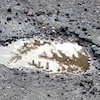
\includegraphics{rd3_9.jpg}

\section{Model training plot}
\label{app:model_plot}

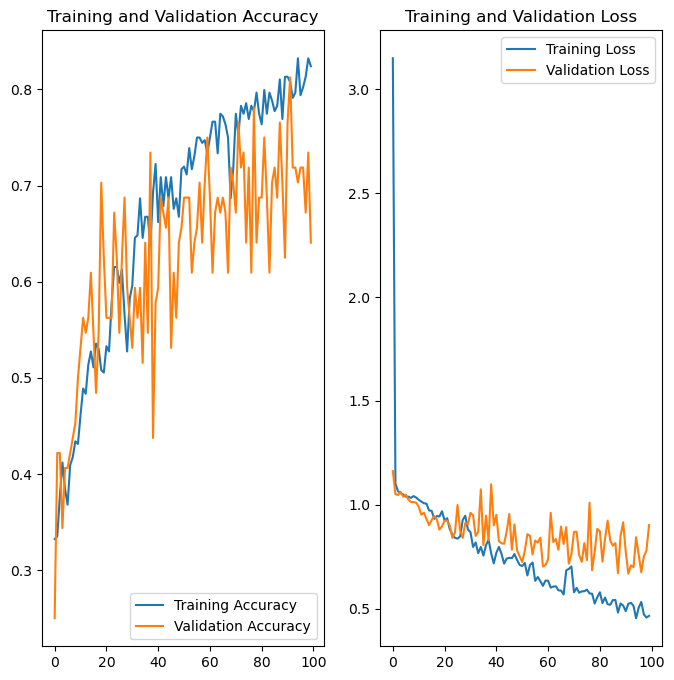
\includegraphics{model_plot.png}

\section{Sample resulting images}
\label{app:result_image}

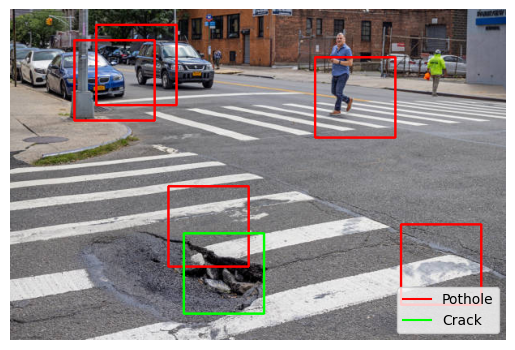
\includegraphics{result_1.png}

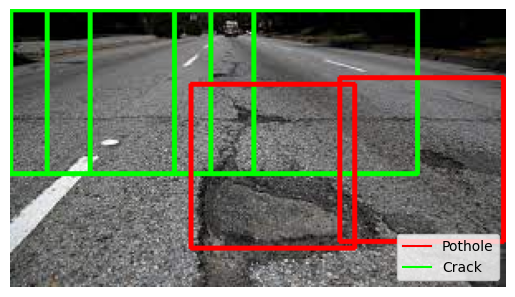
\includegraphics{result_2.png}

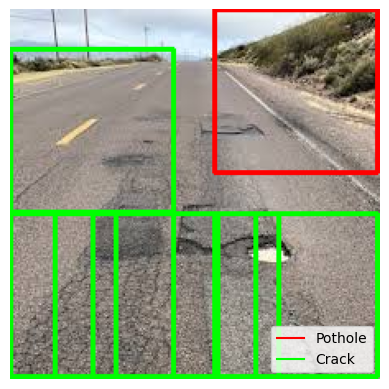
\includegraphics{result_3.png}

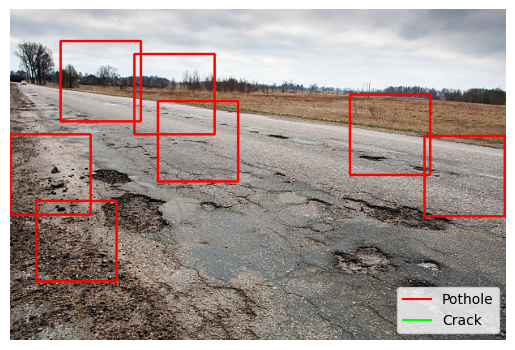
\includegraphics{result_4.png}

\end{document}

% ----------